\newsection

\subsection{BP 2:
 Solitary wave on composite beach (Analytic)}

{\bf Documentation:}

\begin{itemize}
\item PMEL-135, pp 5 \& 30-33 \cite{SynolakisBernard:pmel135}.
\item Problem description \cite{bp-description}.
\item Coastal Hydraulics Laboratory Problem Description \cite{CHLBP2}.
\end{itemize}

\subsubsection{What we did}
\begin{itemize}

\item We solved the shallow water wave equation in Cartesian coordinates with $g = 9.81$ and no friction.
\item To specify the incoming wave from the left boundary of our computational domain we used the first ten seconds of  measurements taken at Gage 4.  After ten seconds the left boundary switched to be a non-reflecting boundary.  This boundary is selected since the end of our computational domain is not the end of the physical wave tank.  
The implementation of these boundary conditions is described in \Sec{bc}.
\item Since the problem is one-dimensional, we solved on a $600 \times 2$ grid with no adaptive mesh refinement.
\item To impose linearization we scaled the incoming wave by $10^{-4}$ to
remove  any nonlinear behavior, then scaled up the gage readings by $10^4$
to compare with the analytical solution.
\end{itemize}

\subsubsection{Gage comparisons}
For these Gage comparisons we ran our code linearly with friction set to zero. 

The results for cases A, B, and C are shown in figures \Fig{bp2A}, \Fig{bp2B}, \Fig{bp2C} respectively where Gage 11 is placed at the vertical wall.

\begin{figure}[ht]
\hfil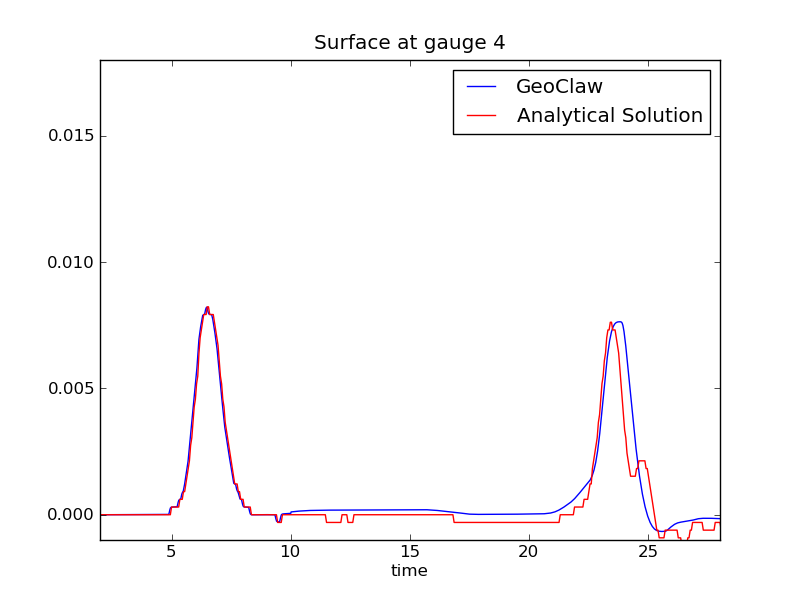
\includegraphics[width=2.8in]{bp2/CaseA/gauge0004fig300.png}\hfil
\hfil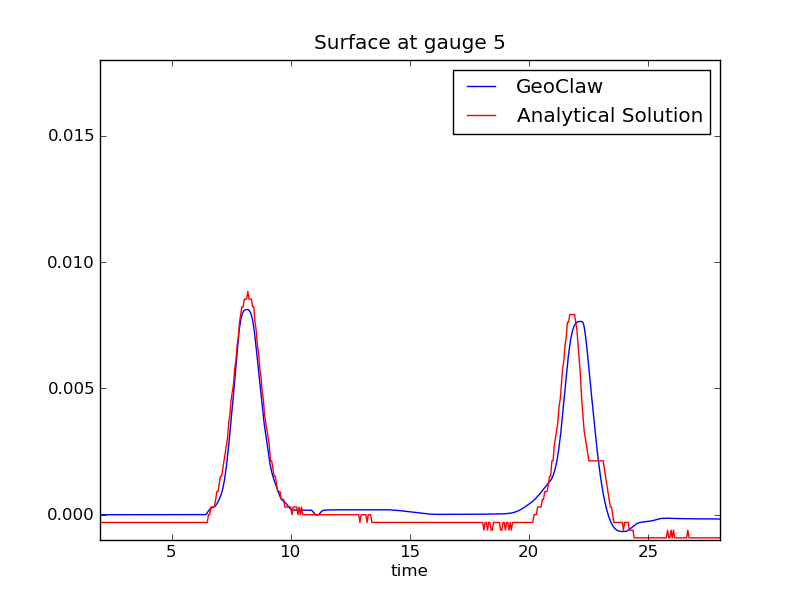
\includegraphics[width=2.8in]{bp2/CaseA/gauge0005fig300.png}\hfil
\vskip 5pt
\hfil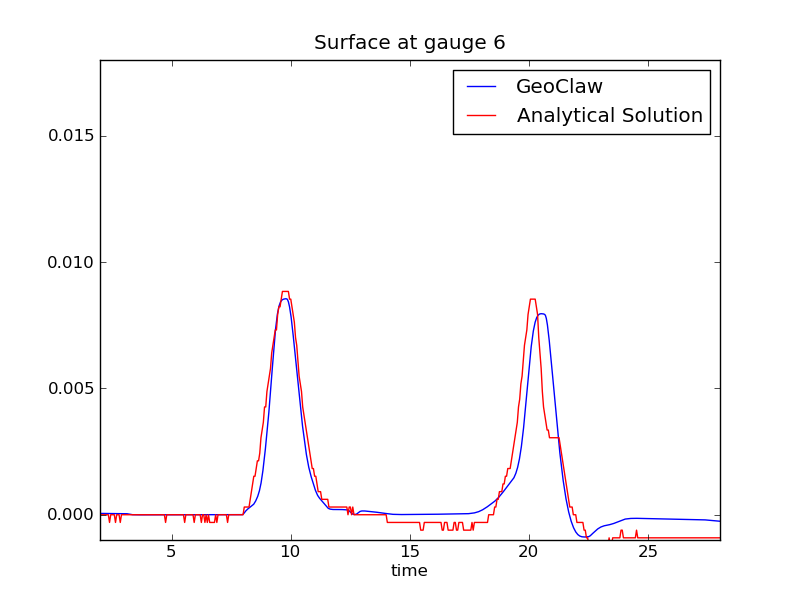
\includegraphics[width=2.8in]{bp2/CaseA/gauge0006fig300.png}\hfil
\hfil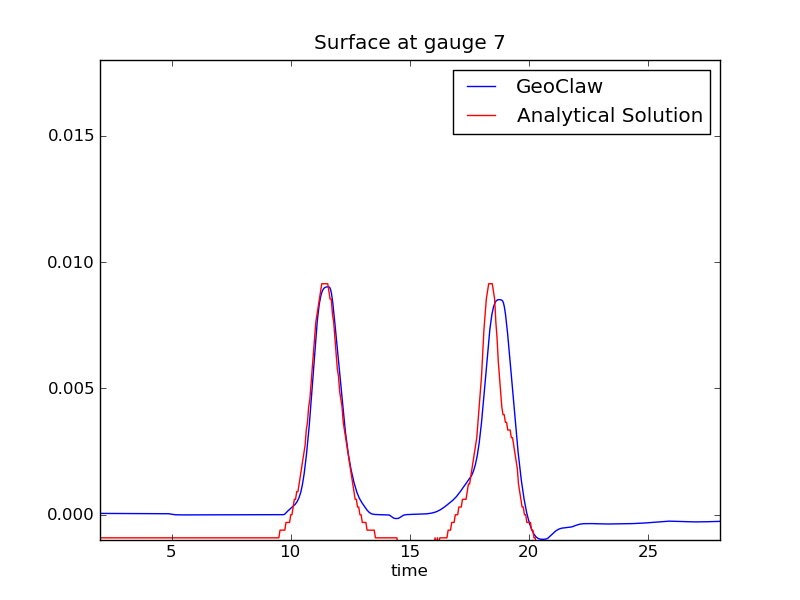
\includegraphics[width=2.8in]{bp2/CaseA/gauge0007fig300.png}\hfil
\vskip 5pt
\hfil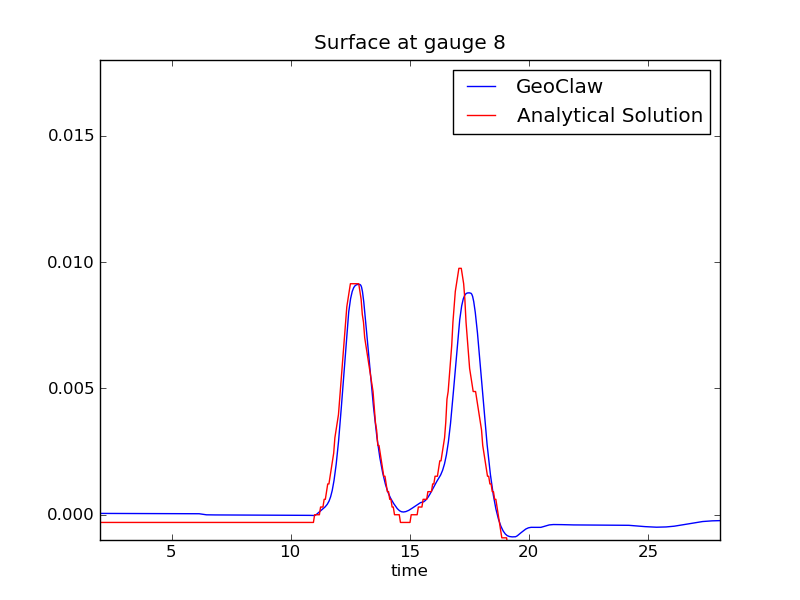
\includegraphics[width=2.8in]{bp2/CaseA/gauge0008fig300.png}\hfil
\hfil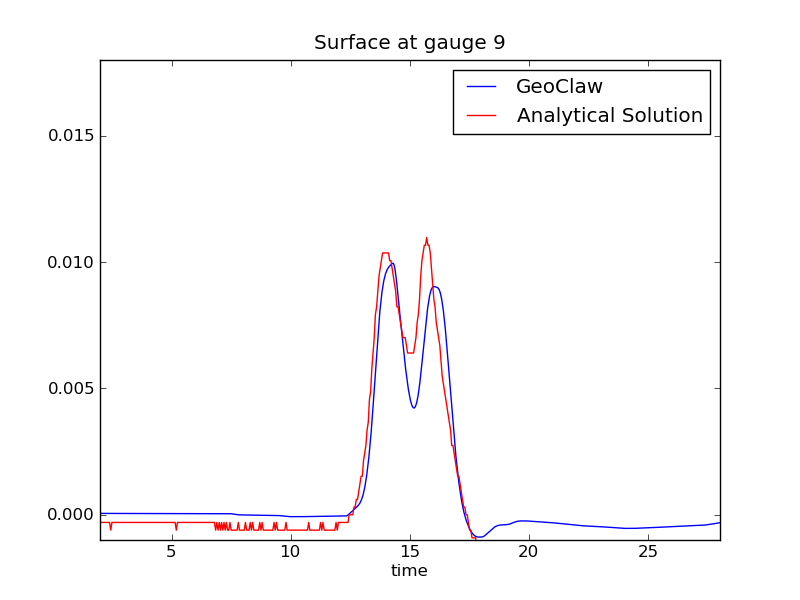
\includegraphics[width=2.8in]{bp2/CaseA/gauge0009fig300.png}\hfil
\vskip 5pt
\hfil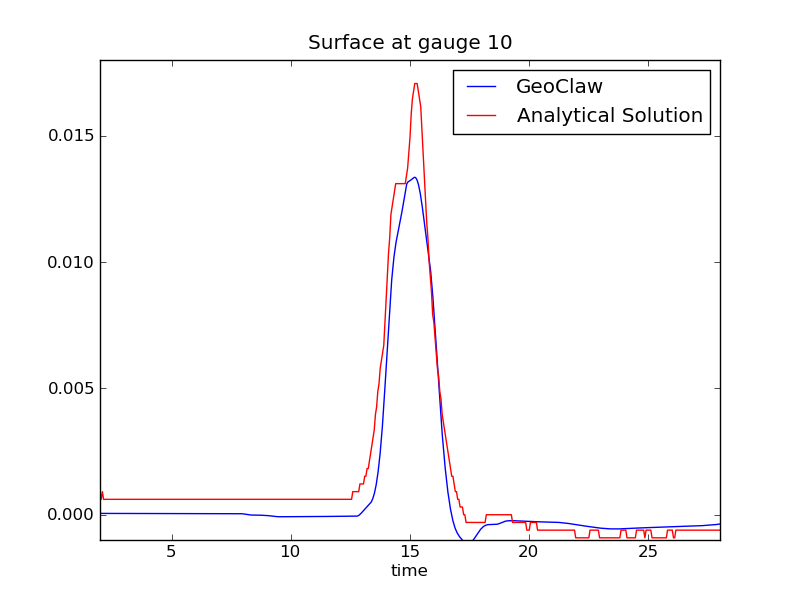
\includegraphics[width=2.8in]{bp2/CaseA/gauge0010fig300.png}\hfil
\hfil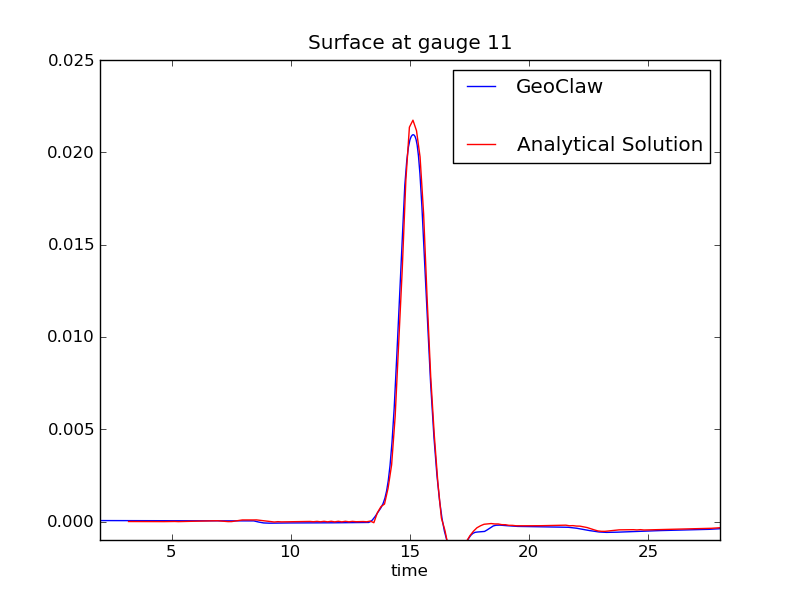
\includegraphics[width=2.8in]{bp2/CaseA/gauge0011fig300.png}\hfil
\caption{\label{fig:bp2A} Case A }
\end{figure}

\begin{figure}[ht]
\hfil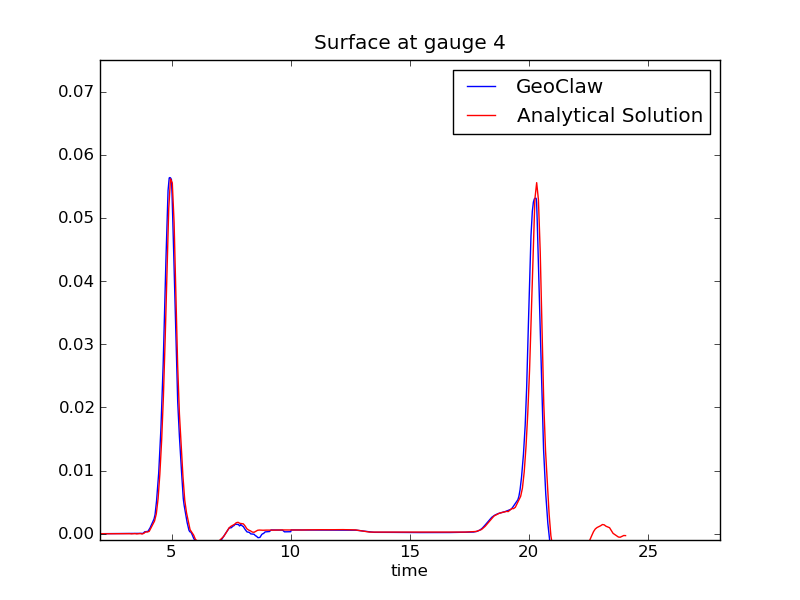
\includegraphics[width=2.8in]{bp2/CaseB/gauge0004fig300.png}\hfil
\hfil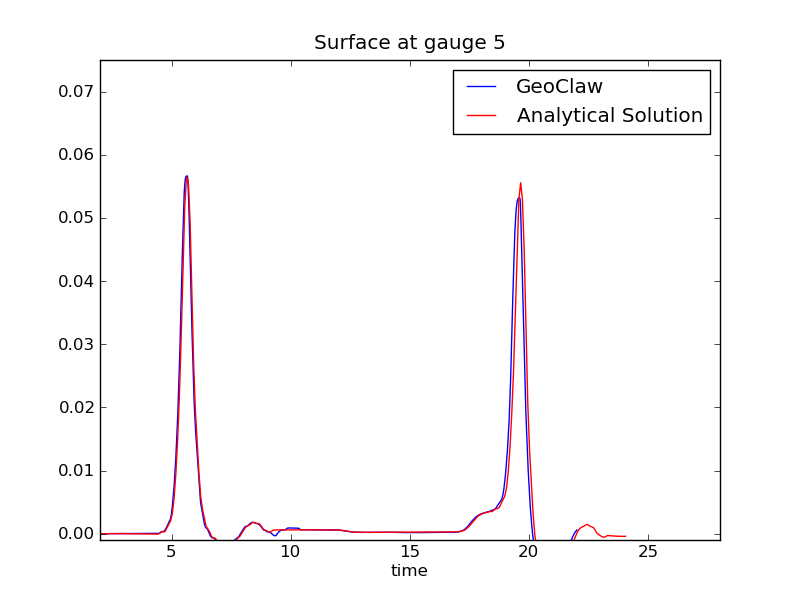
\includegraphics[width=2.8in]{bp2/CaseB/gauge0005fig300.png}\hfil
\vskip 5pt
\hfil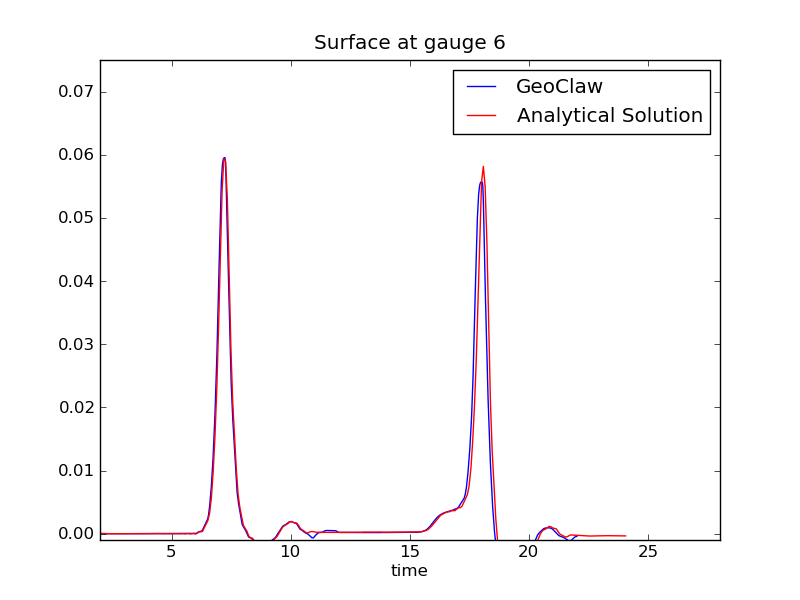
\includegraphics[width=2.8in]{bp2/CaseB/gauge0006fig300.png}\hfil
\hfil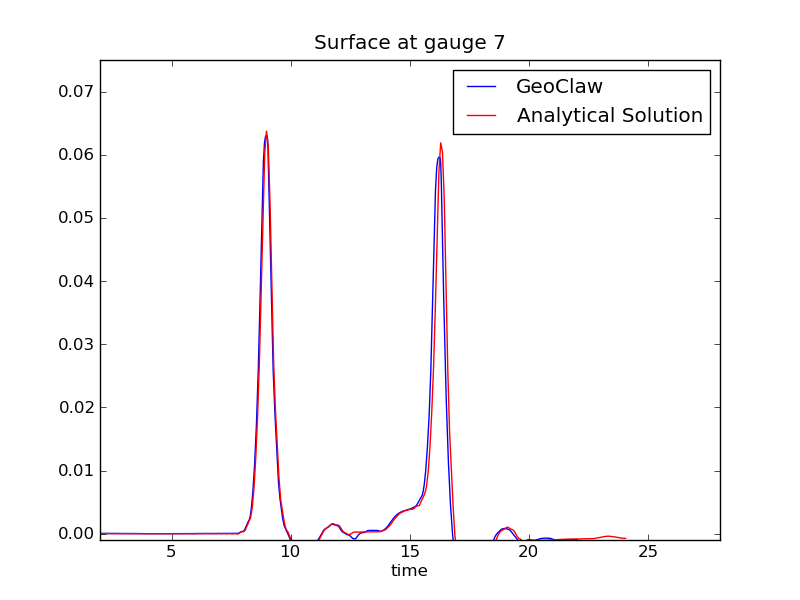
\includegraphics[width=2.8in]{bp2/CaseB/gauge0007fig300.png}\hfil
\vskip 5pt
\hfil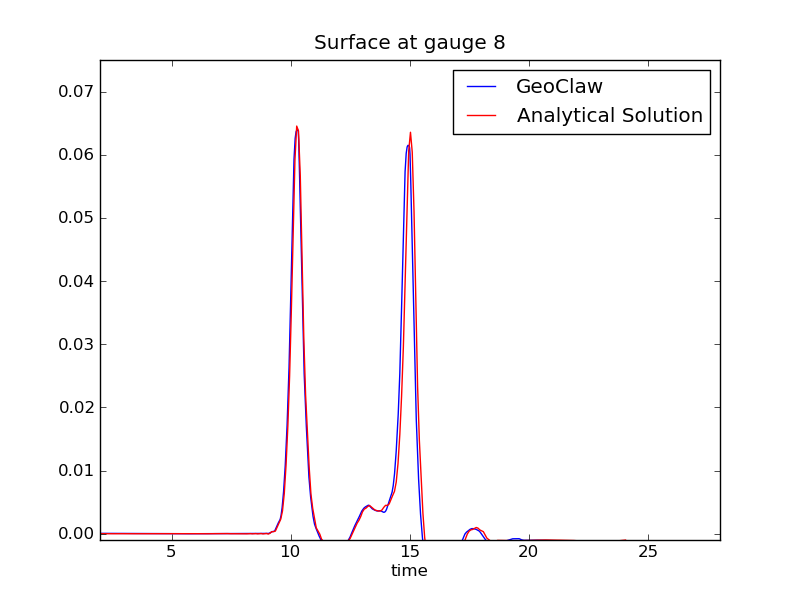
\includegraphics[width=2.8in]{bp2/CaseB/gauge0008fig300.png}\hfil
\hfil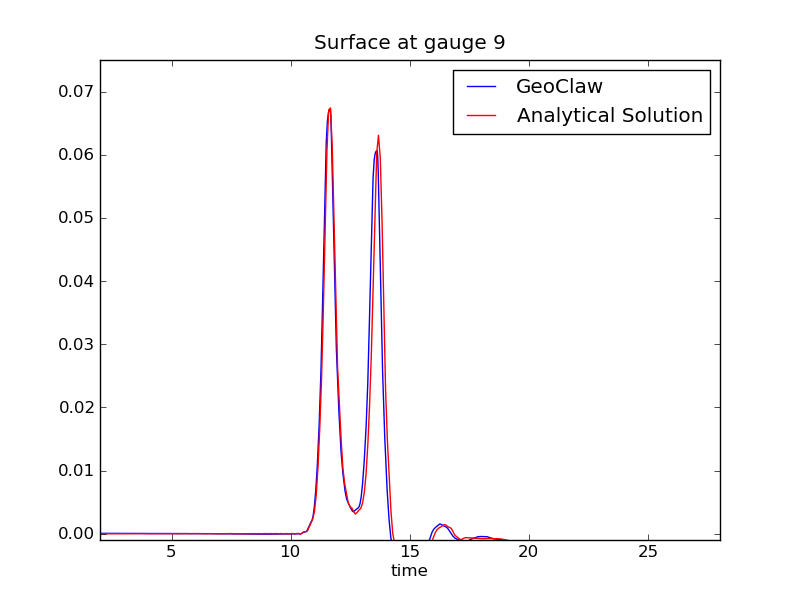
\includegraphics[width=2.8in]{bp2/CaseB/gauge0009fig300.png}\hfil
\vskip 5pt
\hfil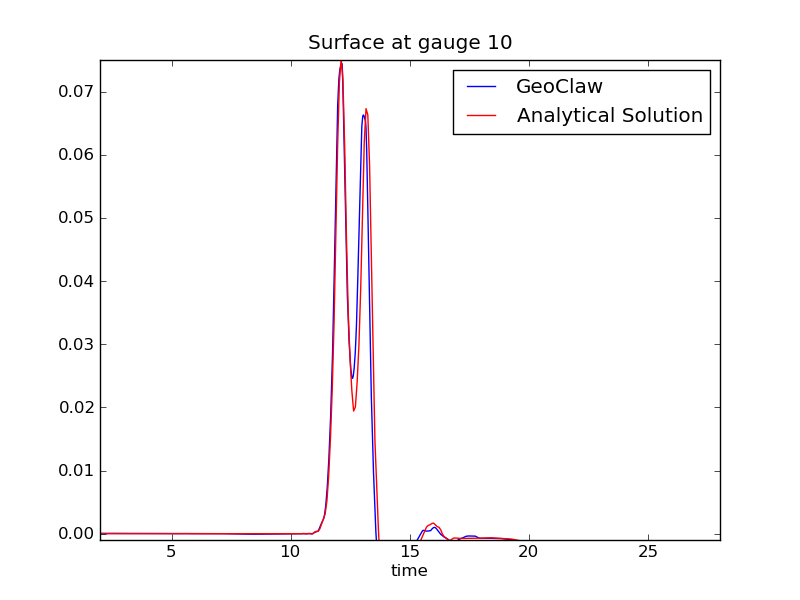
\includegraphics[width=2.8in]{bp2/CaseB/gauge0010fig300.png}\hfil
\hfil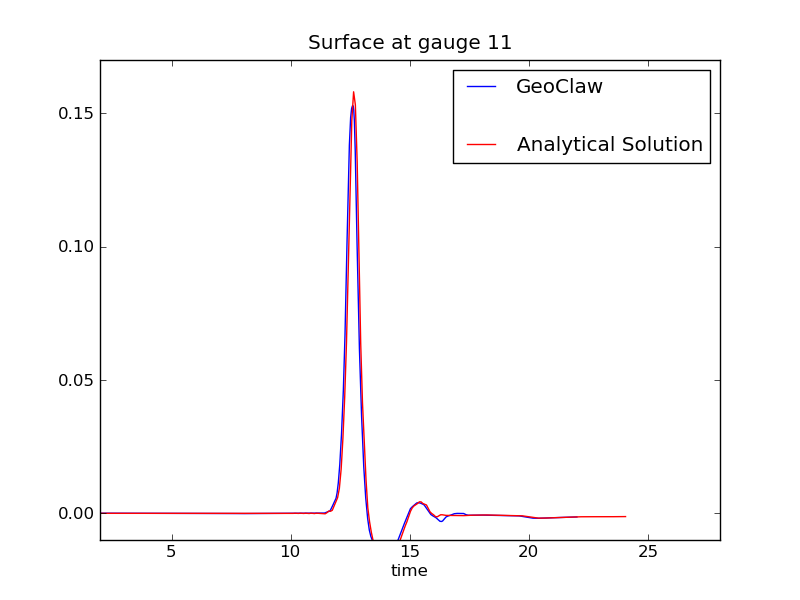
\includegraphics[width=2.8in]{bp2/CaseB/gauge0011fig300.png}\hfil
\caption{\label{fig:bp2B} Case B }
\end{figure}


\begin{figure}[ht]
\hfil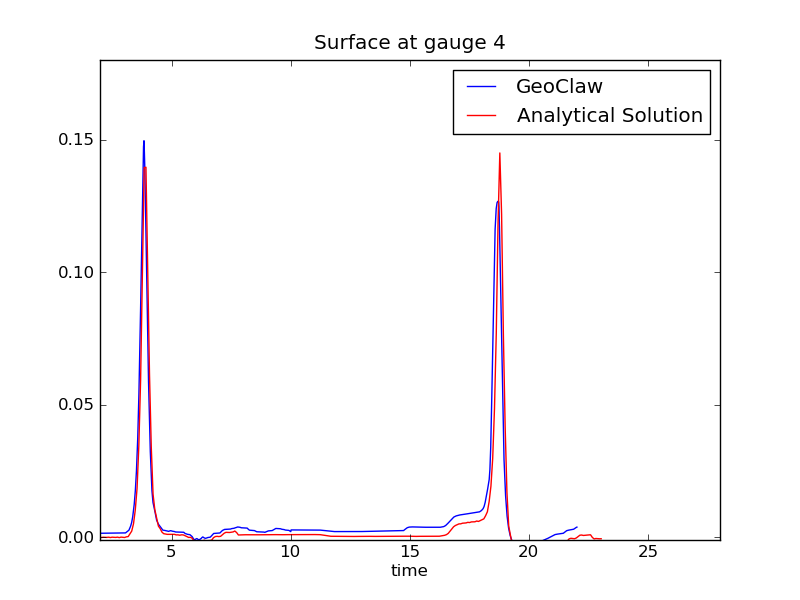
\includegraphics[width=2.8in]{bp2/CaseC/gauge0004fig300.png}\hfil
\hfil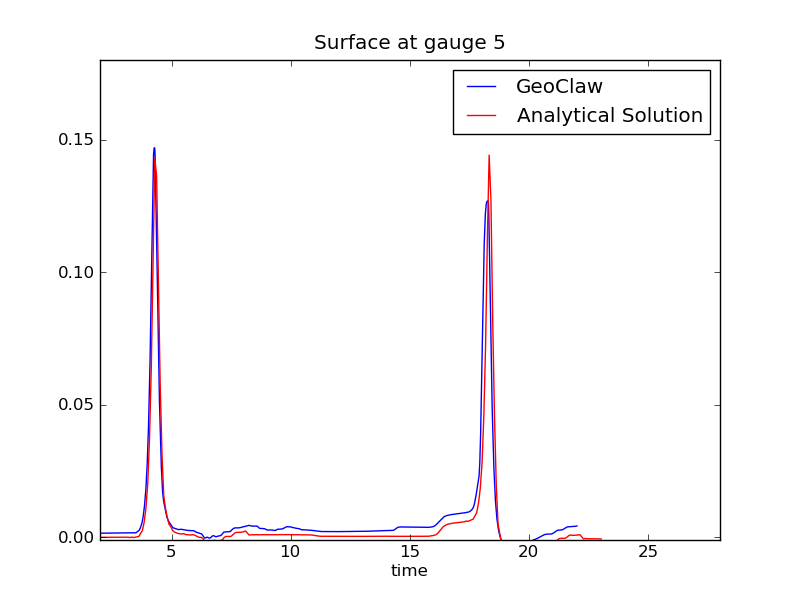
\includegraphics[width=2.8in]{bp2/CaseC/gauge0005fig300.png}\hfil
\vskip 5pt
\hfil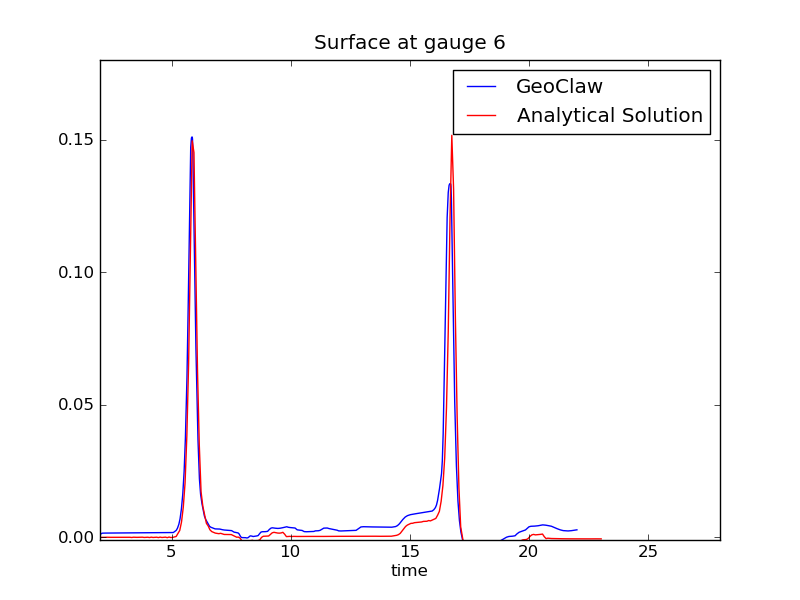
\includegraphics[width=2.8in]{bp2/CaseC/gauge0006fig300.png}\hfil
\hfil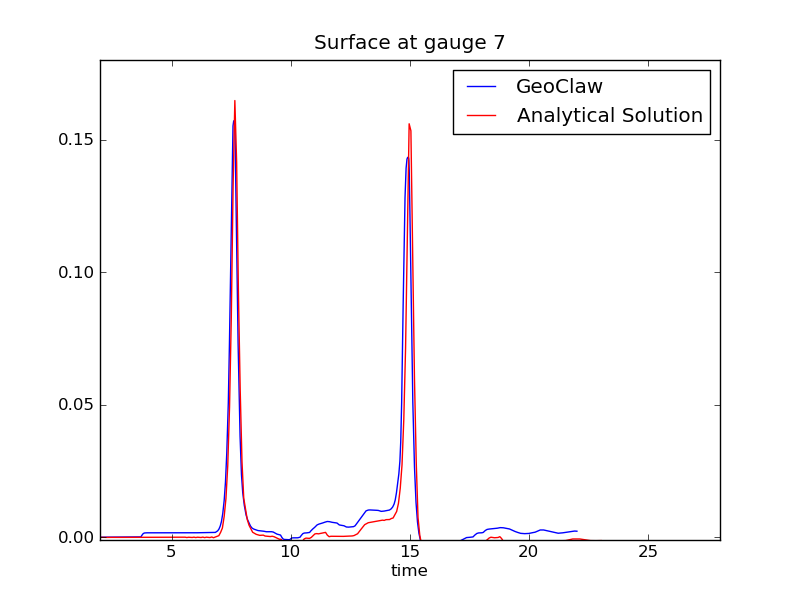
\includegraphics[width=2.8in]{bp2/CaseC/gauge0007fig300.png}\hfil
\vskip 5pt
\hfil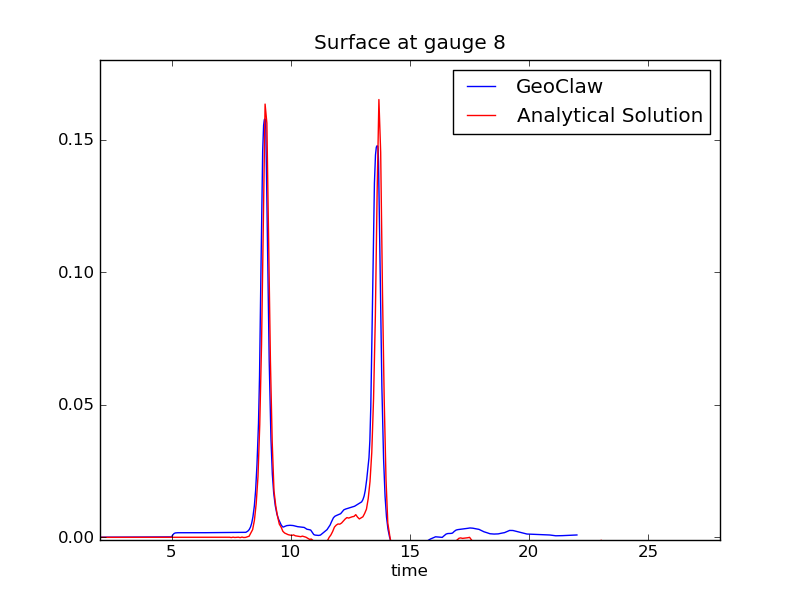
\includegraphics[width=2.8in]{bp2/CaseC/gauge0008fig300.png}\hfil
\hfil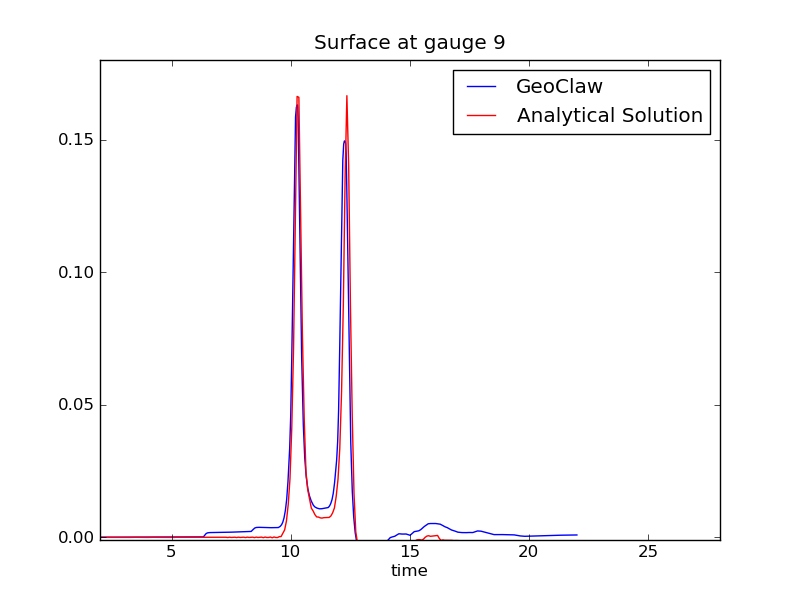
\includegraphics[width=2.8in]{bp2/CaseC/gauge0009fig300.png}\hfil
\vskip 5pt
\hfil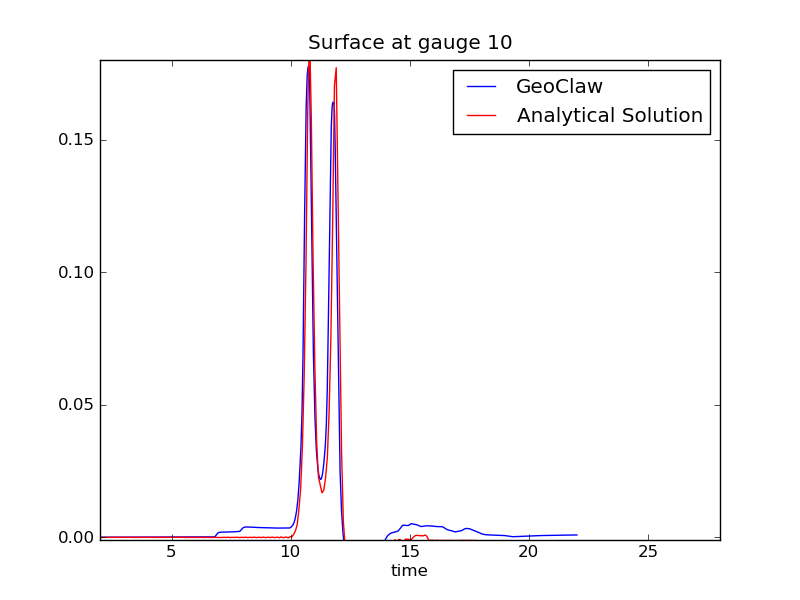
\includegraphics[width=2.8in]{bp2/CaseC/gauge0010fig300.png}\hfil
\hfil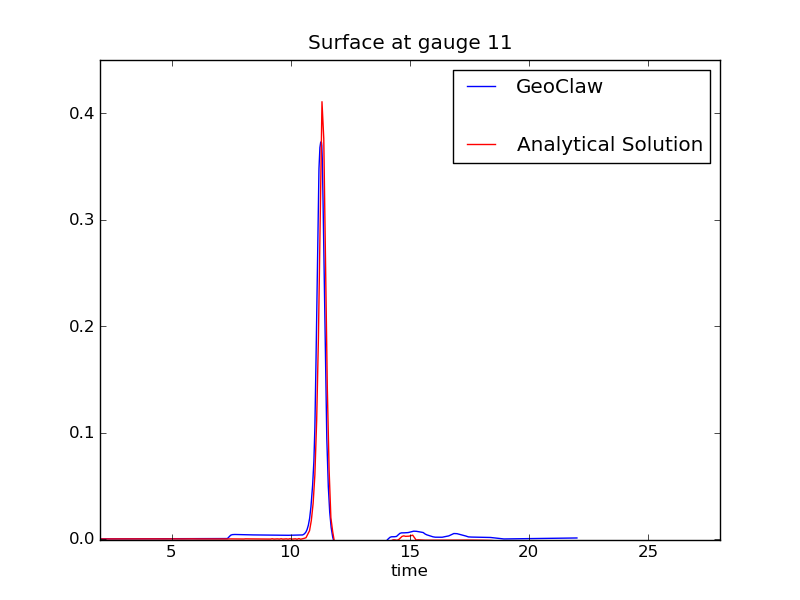
\includegraphics[width=2.8in]{bp2/CaseC/gauge0011fig300.png}\hfil
\caption{\label{fig:bp2C} Case C }
\end{figure}

\subsubsection{Convergence Study}
We performed a test to see how well Clawpack converged to the analytic
solution as we increased the number of grid cells in our computational
domain (using 200, 400, and 600 cells).  
We found that as the number of grid cells was increased,  the computed solution approached the analytic solution.  The convergence plot is shown in \Fig{linearConverge}.

\begin{figure}[ht]
\hfil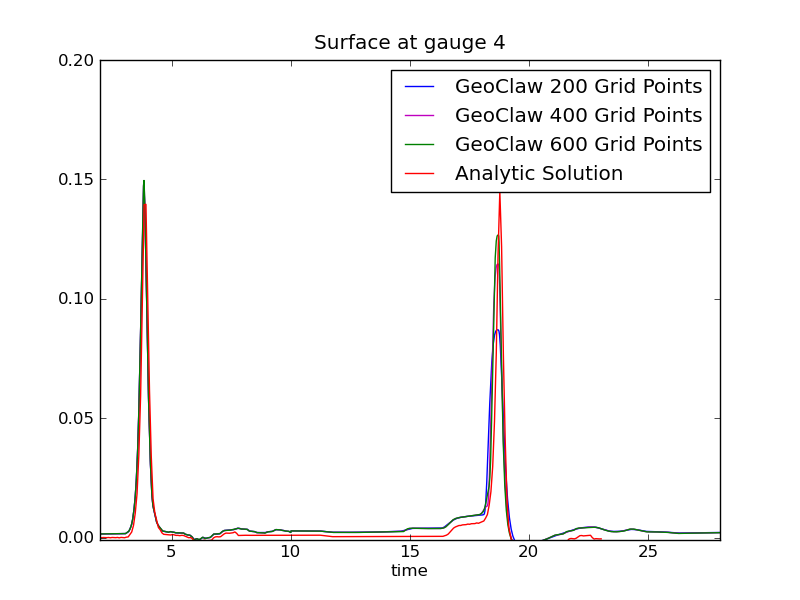
\includegraphics[width=5.8in]{bp2/linearCompare}\hfil
\caption{\label{fig:linearConverge} Convergence Plot for Gage 4 in Case C }
\end{figure}


\subsubsection{Lessons learned}
In this benchmark problem we found that using the analytic solution at Gage 4 as boundary conditions on a shorter domain, starting at gage 4, provided more accurate results than using the wave maker position and a longer domain to model the entire tank.  It appears that a similar assumption is made in the provided analytic solutions, as they match up nearly perfectly with the lab data for the first ten seconds.  

Overall this benchmark problem is a good test for one dimensional codes.  The benchmark problem specifications could be improved by specifying the computational domain and the specific data source that should be used to model the incoming wave. 

